\section{METHOD}
\label{method}
The proposed methods rely on the the geometry induced by the models~\eqref{eq:staticWrench} and~\eqref{wrenchInSensorCoordinates}.

\subsection{The geometry of the raw measurements}
\label{subsec:geometry}
First, observe that
\[ \text{rank}(M) = 3 .\]
As a consequence, all wrenches $w$ belong to the three-dimensional subspace given by the $\operatorname{span}{(M)} \subset \mathbb{R}^6$. In view of this,
we can state the following lemma.


\lemma{1}{All raw measurements $r$ belong to a three dimensional affine space,  i.e. there exist a point $r_m \in \mathbb{R}^6$, an orthonormal basis 
$U_1 \in \mathbb{R}^{6 \times 3}$, and for each $r \in \mathbb{R}^6$ a vector $\lambda \in \mathbb{R}^3$ such that 
\begin{IEEEeqnarray}{RCL}
 \label{decompositionMeasurements}
 r &=& r_m + U_1 \lambda.
\end{IEEEeqnarray}
Also, the vector $\lambda$ belongs to a three-dimensional ellipsoid.
}
\begin{proof}
From \eqref{wrenchInSensorCoordinates} and \eqref{eq:staticWrench}, one has:
\begin{equation}
\label{rFromModel}
r  = |g|C^{-1} M \hat{g} + o,
\end{equation}
where $\hat{g} := g/|g|$.
The matrix $C^{-1}M \in \mathbb{R}^{6\times3}$ is of rank~$3$.
Consequently, all raw measurements $r$ belong to an affine three-dimensional space 
defined by the point $o$ and the basis of $\operatorname{span}{(C^{-1}M)}$.
Now, define $P \in \mathbb{R}^{3 \times 6}$ as the projector of $r$ onto $\operatorname{span}{(C^{-1}M)}$.
 Then, the projection $p \in \mathbb{R}^3$ of $r$ onto this span is given by  
\begin{IEEEeqnarray}{RCL}
  p &=& Pr = |g|PC^{-1} M \hat{g} + Po.
\end{IEEEeqnarray} 
By considering all possible orientations of the sensor's frame~$\mathcal{S}$, then the gravity direction $\hat{g}$ spans the unit sphere. 
Consequently, the vector $p$ belongs to the \textit{span of the unit sphere applied to the linear transformation $|g|PC^{-1} M$}, 
i.e. an \textit{ellipsoid centered at the point $Po$}. This in turn implies that when decomposing the vector $r$ as in~\eqref{decompositionMeasurements},
the vector~$\lambda$ necessarily belongs to a three-dimensional ellipsoid.
\end{proof}

To provide the reader with a better comprehension of the above lemma, assume that $r \in \mathbb{R}^{3}$ and that the affine subspace is 
a plane, i.e. a two-dimensional space. 
As a consequence, all measurements belong to an ellipse lying on this plane -- see Figure~\ref{imageWithPlane}. Observe also that given a point 
$\lambda \in \mathbb{R}^2$ on the plane and expressed w.r.t. the basis $U_1$, the relationship~\eqref{decompositionMeasurements} provides with the components of this point in the space 
$\mathbb{R}^3$.
\begin{figure}
\vspace{2em}
\centering
    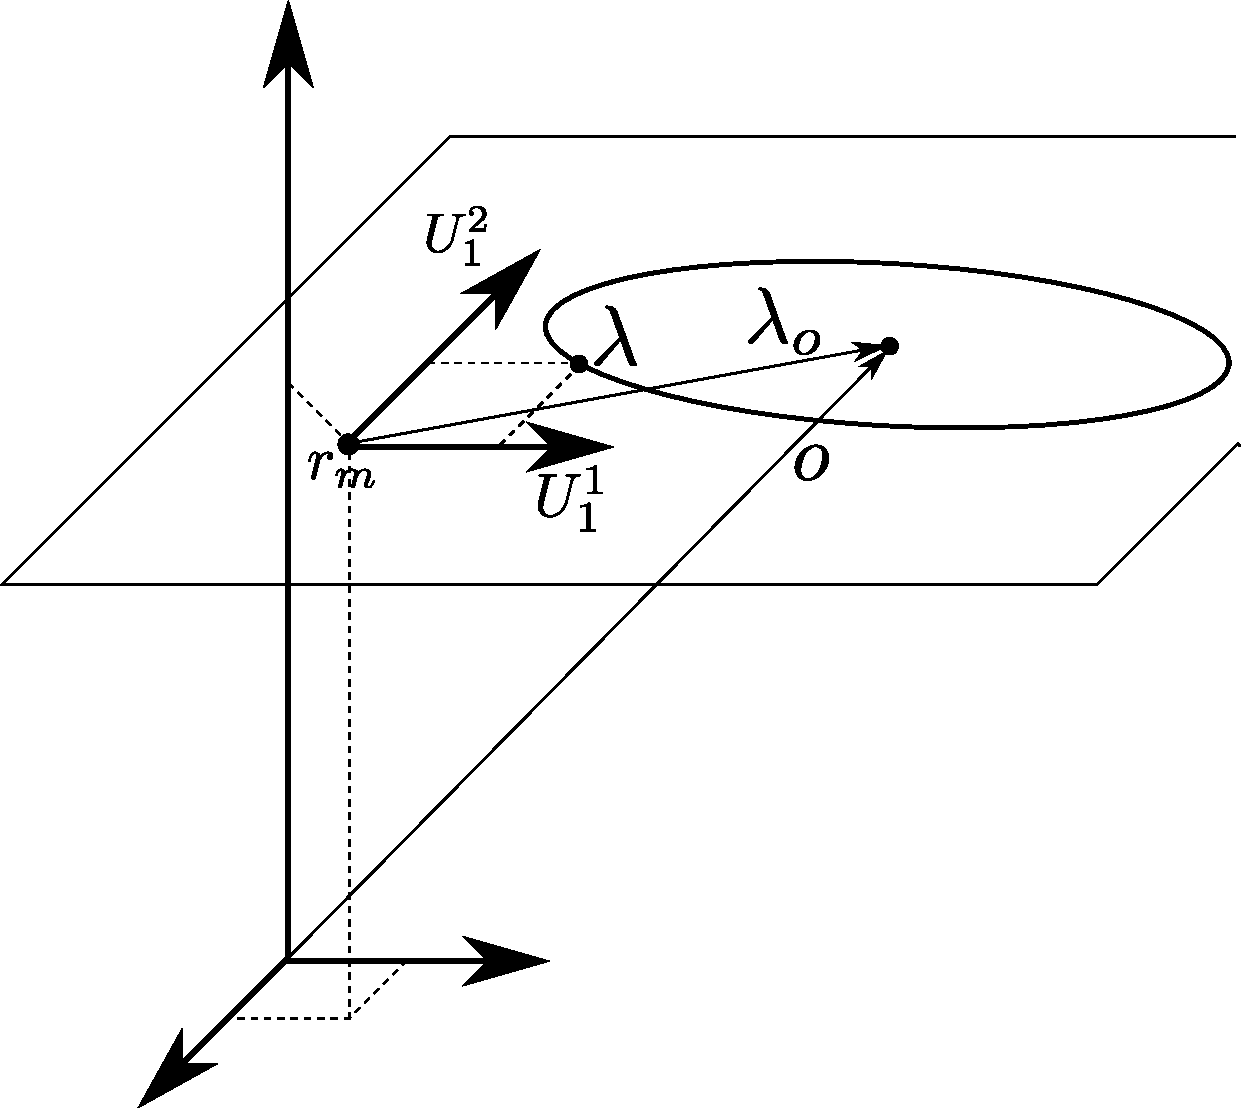
\includegraphics[width=0.45\textwidth]{images/imageWithPlane.pdf}
    \caption{Example when $r \in \mathbb{R}^3$ and $U_1 = (U_1^1,U_1^2) \in \mathbb{R}^{3 \times 2}$. }
    \label{imageWithPlane}
\end{figure}
By leveraging on the above lemma, the next two sections propose a method to estimate the sensor's offset and calibration matrix.

\subsection{Method for estimating the sensor's offset}
\label{offsetEstimationTechnique}

Assume that one is given with a set of measurements $(r_i,g_i)$ with $i \in \{1 \cdots N \}$ corresponding to several body's static orientations. 
Then, let 
us show how we can obtain the basis $(r_m,U_1)$ in~\eqref{decompositionMeasurements} associated with all measurements $r_i$, and how this basis
can be used for estimating the offset $o$.

Observe that the point $r_m$ can be chosen as any point that belongs to the affine space. Then, 
a noise-robust choice for this point is given by the mean value of the measurements~$r_i$,
\begin{IEEEeqnarray}{RCL}
 r_m &=& \frac{1}{N} \sum\limits_{i=1}^N r_i.
\end{IEEEeqnarray}
An orthonormal basis $U_1$ can be then obtained by applying the singular value decomposition on the matrix resulting from the difference between  
all measurements and $r_m$, i.e.
\begin{IEEEeqnarray}{RCL}
%  R &:=& 
 (\tilde{r}_1, \cdots, \tilde{r}_n) = USV^\top,  
\end{IEEEeqnarray}
where 
% $R \in \mathbb{R}^{6\times N}$,  and 
\[\tilde{r}_i := r_i - r_m,\] and $U \in \mathbb{R}^{6\times6}$, $S \in \mathbb{R}^{ 6 \times N}$, $V \in \mathbb{R}^{N\times N}$ are 
the (classical) matrices obtained from the singular value decomposition. 
Note that
only the first three elements on the diagonal of$~S$ are (significantly) different from zero
since all measurements~$r_i$ belong to a three dimensional subspace. Consequently, (an estimate of) the orthonormal basis $U_1$ is given by the first
three columns of the matrix~$U$. 
 
With $(r_m,U_1)$ in hand, the offset $o$ can be easily estimated.
First, note that equation \eqref{decompositionMeasurements} holds for all points belonging to the three dimensional space.
Hence, it holds also for the offset $o$ being the center of the ellipsoid (see Figure~\ref{imageWithPlane}), i.e. 
\begin{equation}
\label{eq:offsetInPlane}
o = r_m + U_1 \lambda_o .
\end{equation}
Then to estimate the offset $o$ belonging to $\mathbb{R}^6$, we can estimate the coordinates $\lambda_o$ in the subspace $\mathbb{R}^3$. In view of $U_1^\top U_1 = I_3$, multiplying
the above equation times $U_1^\top$ yields
\begin{equation}
\lambda_o := U^{\top}_1(o-r_m).
\end{equation}
Now, by subtracting $r_m$ from \eqref{rFromModel} and multiplying the resulting equation by $U_1^\top$, one has
\begin{equation}
 \label{rFromModel1}
 U^{\top}_1\tilde{r}_i  = Kg_i + \lambda_o,
\end{equation}
where 
% $g_i$ is the measurement of the gravity acceleration provided by the accelerometer, and 
\[K := U^\top_1C^{-1}M \quad \text{and} \quad \lambda_o \] are the unknowns
in the above equation. In view of~\eqref{eq:kroneckerVec} the equation~\eqref{rFromModel1} can be written by stacking the obtained vectors for all measurements as
\begin{IEEEeqnarray}{RCLRCL}
 \bar{r}  &=& \Gamma x,  \IEEEyessubnumber \label{eqForOffset} \\
\bar{r} &:=& 
 \begin{pmatrix}
  \tilde{r}^\top_1U_1, && \cdots, && \tilde{r}^\top_NU_1
 \end{pmatrix}^\top &\in& \mathbb{R}^{3N\times 1},  \IEEEyessubnumber \\ 
 \Gamma &:=& 
 \begin{pmatrix}
  g^\top_1 \otimes I_3, I_3 \\
  . \\
  . \\
  g^\top_N \otimes I_3, I_3
 \end{pmatrix}&\in& \mathbb{R}^{3N\times 12},  \IEEEyessubnumber \\
 x &:=& 
 \begin{pmatrix}
  \text{vec}(K) \\
  \lambda_o
 \end{pmatrix}&\in& \mathbb{R}^{12\times 1}.\IEEEyessubnumber
\end{IEEEeqnarray}
Solving the equation~\eqref{eqForOffset} for the unknown $x$ in the least-square sense provides with an estimate 
$\hat{\lambda}_o  \in \mathbb{R}^3$ of $\lambda_o$. To obtain the coordinates of this point w.r.t. the six-dimensional space, i.e. the raw measurements space,
we apply the transformation~\eqref{eq:offsetInPlane} as follows:
\[
\hat{o} = r_m + U_1 \hat{\lambda}_o .
\]

\subsection{Method for estimating the  sensor's calibration matrix}
\label{calibrationMatrixEstimation}

In this section, we assume no offset, i.e. $o = 0$, which means that this offset has already been estimated
by using one of the existing methods in the literature 
or by using the method described in the previous section. Consequently, the relationship between the set of measurements 
$(r_i,g_i)$ 
% with $i \in \{1 \cdots N \}$
and the body's inertial characteristics, i.e. mass and center of mass, is given by
\begin{equation}
% \label{rawMeasurementsNoOffset}
Cr_i =  Mg_i \nonumber.
% =  {C} \left( \rawval +  {o_r} \right)
\end{equation} 
In addition, we also assume that the body's inertial characteristics can be modified by adding sample masses at specific relative positions w.r.t. the
sensor frame $\mathcal{S}$. As a consequence, the matrix $M$ in the above equation is replaced by $M_j$, i.e.
\begin{equation}
\label{rawMeasurementsNoOffsetSeveralDataSets}
Cr^j_i =  M_jg^j_i ,
% =  {C} \left( \rawval +  {o_r} \right)
\end{equation} 
where $j$ indicates that new inertial
characteristics have been obtained by adding sample masses. Observe that $M_j$ can then be decomposed as follows
\begin{IEEEeqnarray}{RCCRCL}
 \label{MknownUnkwn}
 M_j &:= &M_b& + &M^j_a& \nonumber \\
    &=& m
\begin{pmatrix}
I_3 \\
c \times 
\end{pmatrix}&
+ &m^j_a
\begin{pmatrix}
I_3 \\
c^j_a \times 
\end{pmatrix}&,  \nonumber
\end{IEEEeqnarray}
where $(m^j_a,c^j_a)$ are the mass and the vector of the center of mass, expressed w.r.t. the sensor frame $\mathcal{S}$, of the added mass.
In the above equation, $M_b$ is unknown but $M^j_a$ is assumed to be known.

In light of the above, we assume to be given with several data sets 
\begin{IEEEeqnarray}{RCL}
 \label{dataSets}
 R_j := (r^j_1, \cdots,r^j_{N_j}) \in \mathbb{R}^{6\times N_j}, \IEEEyessubnumber \\
 G_j := (g^j_1, \cdots,g^j_{N_j}) \in \mathbb{R}^{3\times N_j} ,\IEEEyessubnumber 
\end{IEEEeqnarray}
associated with $N_D$ different $(m^j_a,c^j_a)$. Given~\eqref{rawMeasurementsNoOffsetSeveralDataSets} and~\eqref{dataSets},
the measurements associated with the $jth$ data set can be compactly written as
\begin{IEEEeqnarray}{RCL}
CR_j - M_bG_j&=&   M^j_aG_j. \nonumber
% =  {C} \left( \rawval +  {o_r} \right)
\end{IEEEeqnarray} 
The matrices $C$ and $M_b$ are unknown. Then, in view of~\eqref{eq:kroneckerVec} the above equation can be written for all data sets as follows
\begin{IEEEeqnarray}{RCLRLL}
 \Theta x &=& \beta,  \IEEEyessubnumber \label{equationForEstimatingC} \\
 x &:=& 
 \begin{pmatrix}
  \text{vec}(C) \\
  m \\
  mc
 \end{pmatrix},
 &\in& \mathbb{R}^{40\times 1},  
 \IEEEyessubnumber \\ 
 \Theta &:=& 
 \begin{pmatrix}
  R^\top_1 \otimes I_6, \ -(G^\top_1 \otimes I_6)H  \\
  . \\
  . \\
  R^\top_{N_D} \otimes I_6, \ -(G^\top_{N_j} \otimes I_6)H
 \end{pmatrix},
 &\in& \mathbb{R}^{6N_T\times 40},
 \IEEEyessubnumber \IEEEeqnarraynumspace \\
 \beta &:=& 
 \begin{pmatrix}
  \text{vec}(M^1_a G_1)   \\
  . \\
  . \\
  \text{vec}(M^{N_D}_a G_1) 
 \end{pmatrix},
 &\in& \mathbb{R}^{40\times 1}.
 \IEEEyessubnumber
\end{IEEEeqnarray}
with \[N_T = \sum\limits_{j=1}^{N_D} N_j,\] i.e. the number of all measurements, and the matrix $H~\in~\mathbb{R}^{18\times4}$ a properly chosen permutator such that 
\[\text{vec}(M_b) = H
 \begin{pmatrix}
  m \\
  mc
 \end{pmatrix}.\]
To find the calibration matrix $C$, we have to find the solution~$x$ to the equation~\eqref{equationForEstimatingC}. 
The uniqueness of this solution is characterized by the following lemma.

\lemma{2}{
A necessary condition for the uniqueness of 
the solution $x$ to the equation~\eqref{equationForEstimatingC} is that the number of data sets 
% taken for different center of masses
% of the modified body
must be greater 
than two, i.e.
\begin{IEEEeqnarray}{rcl}
 \label{necessityForWellPosedenessC}
 N_D \geq 3.
\end{IEEEeqnarray}
}

\begin{figure}[t]
\centering
\subfloat[Dataset 1: no added mass]{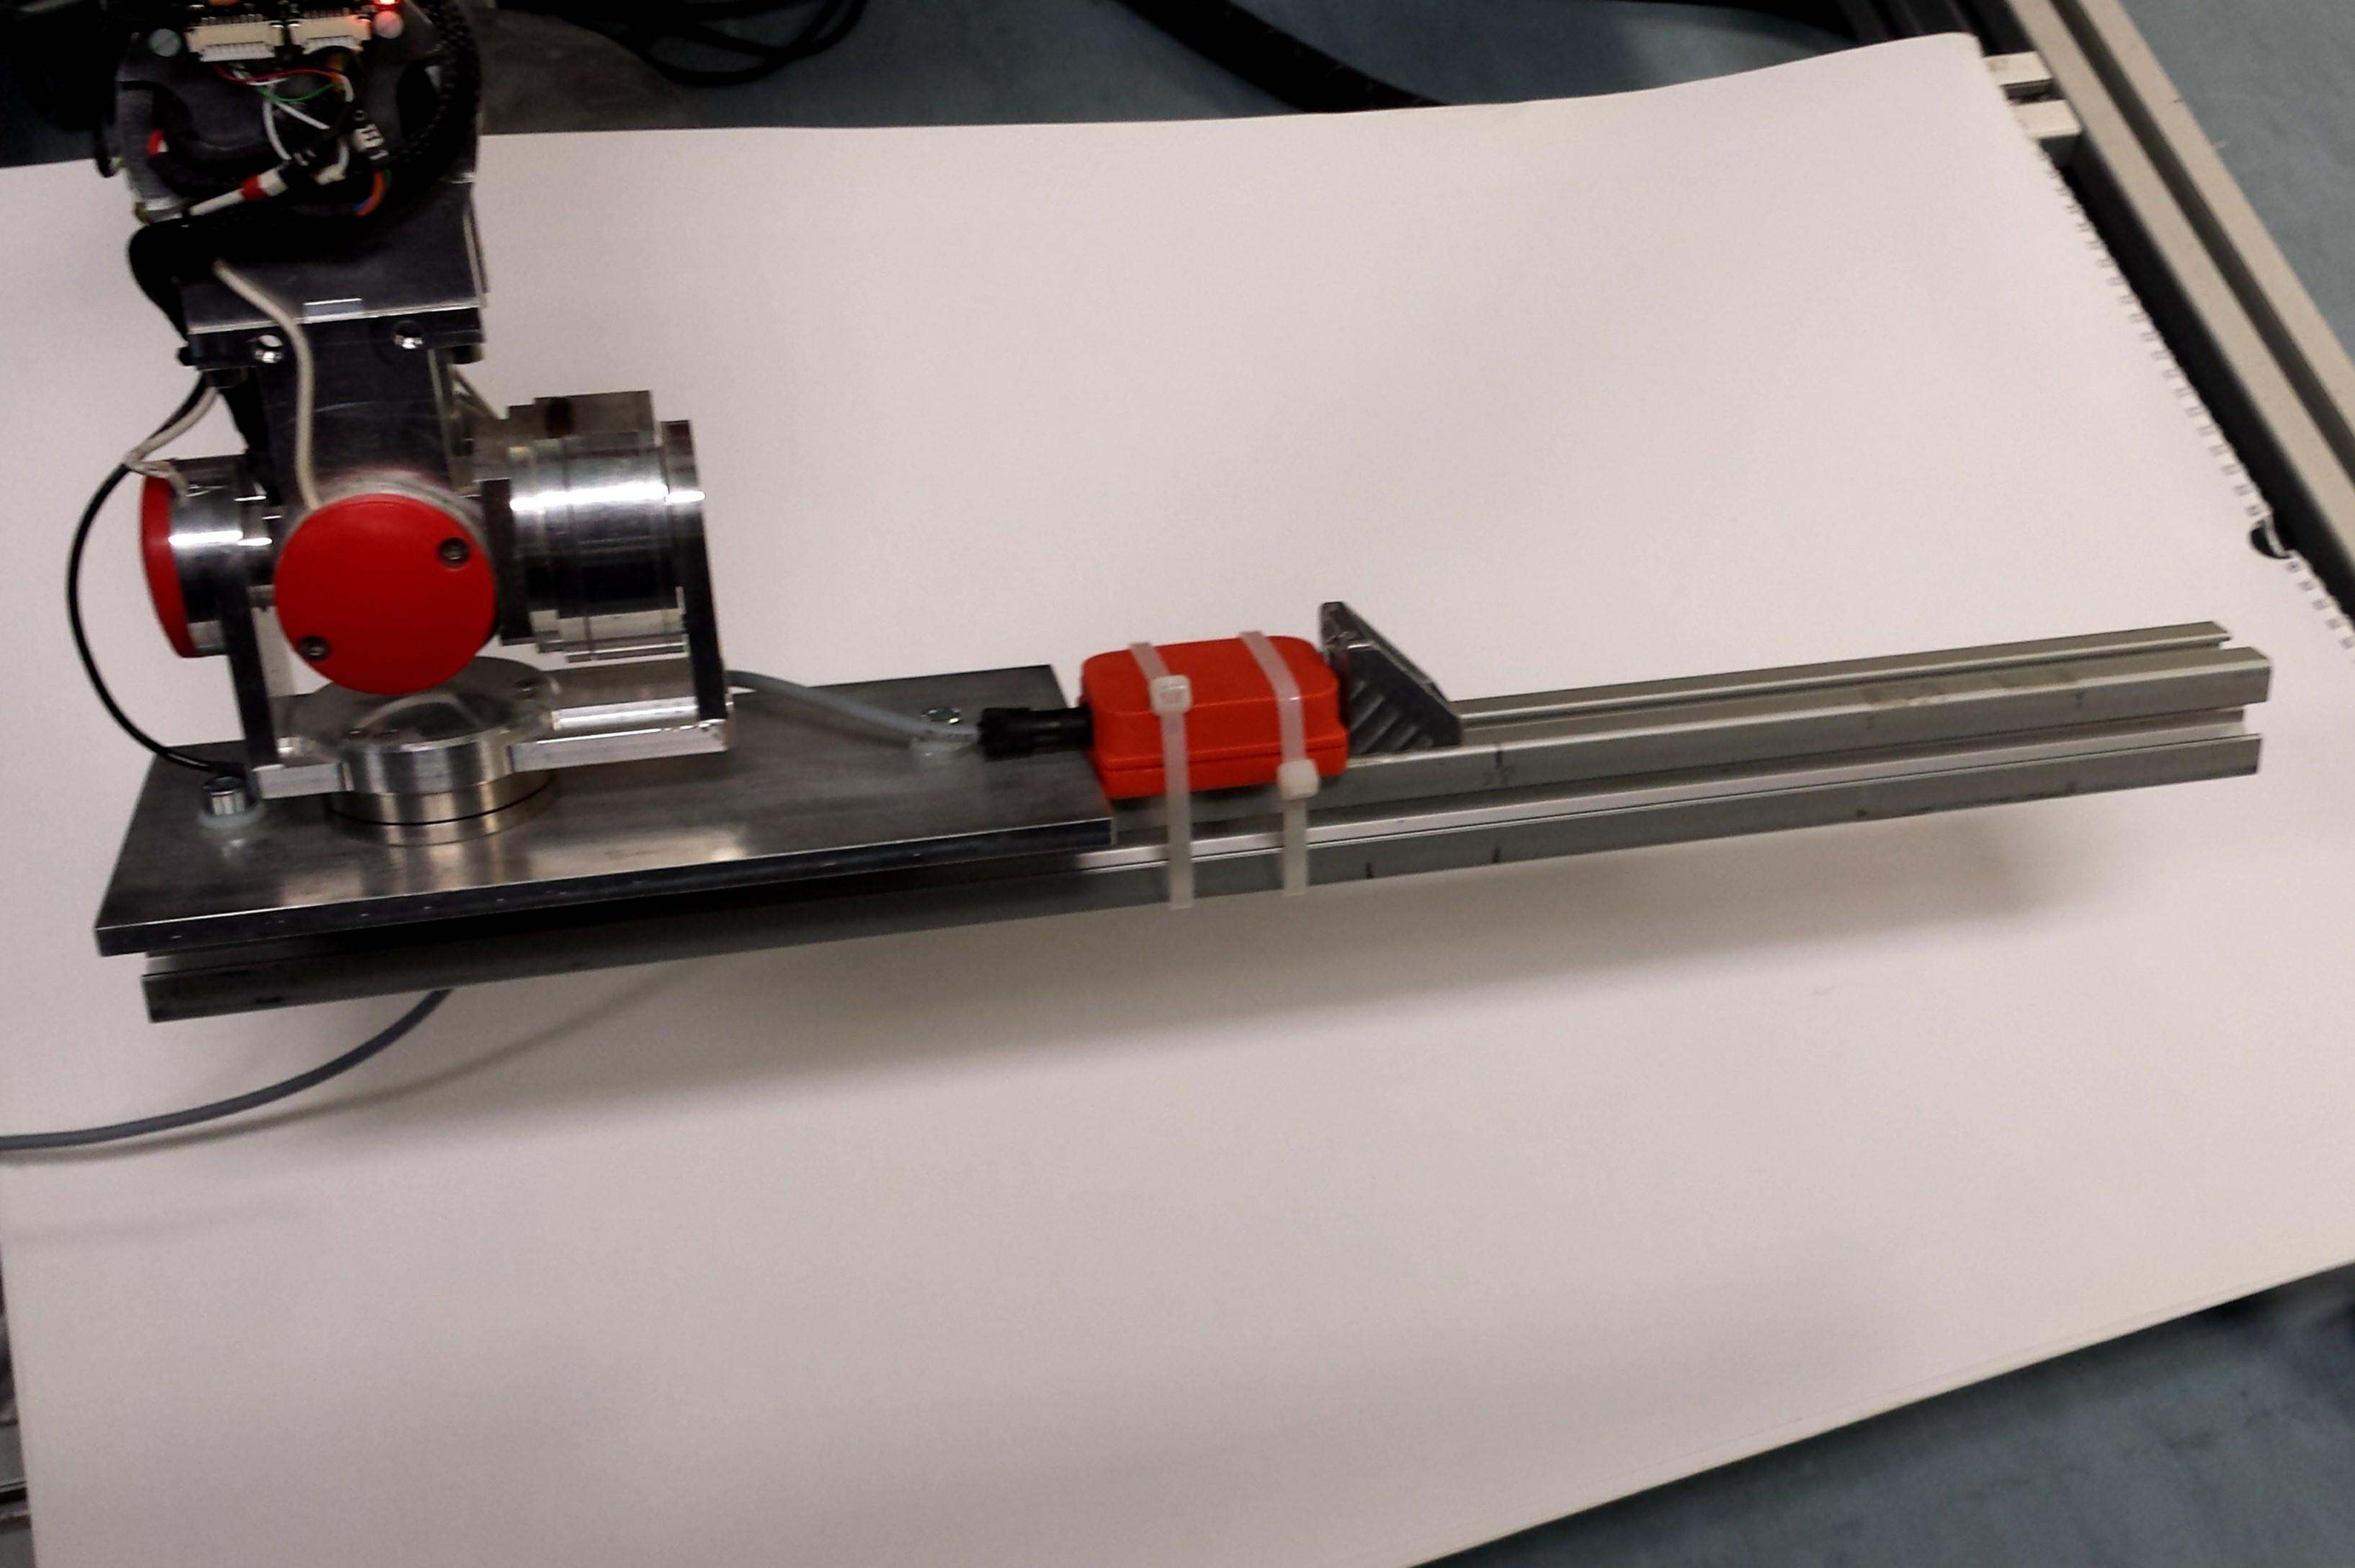
\includegraphics[width=0.22\textwidth]{images/dataset0107.pdf}
\label{fig:dataset1}}
\subfloat[Dataset 2]{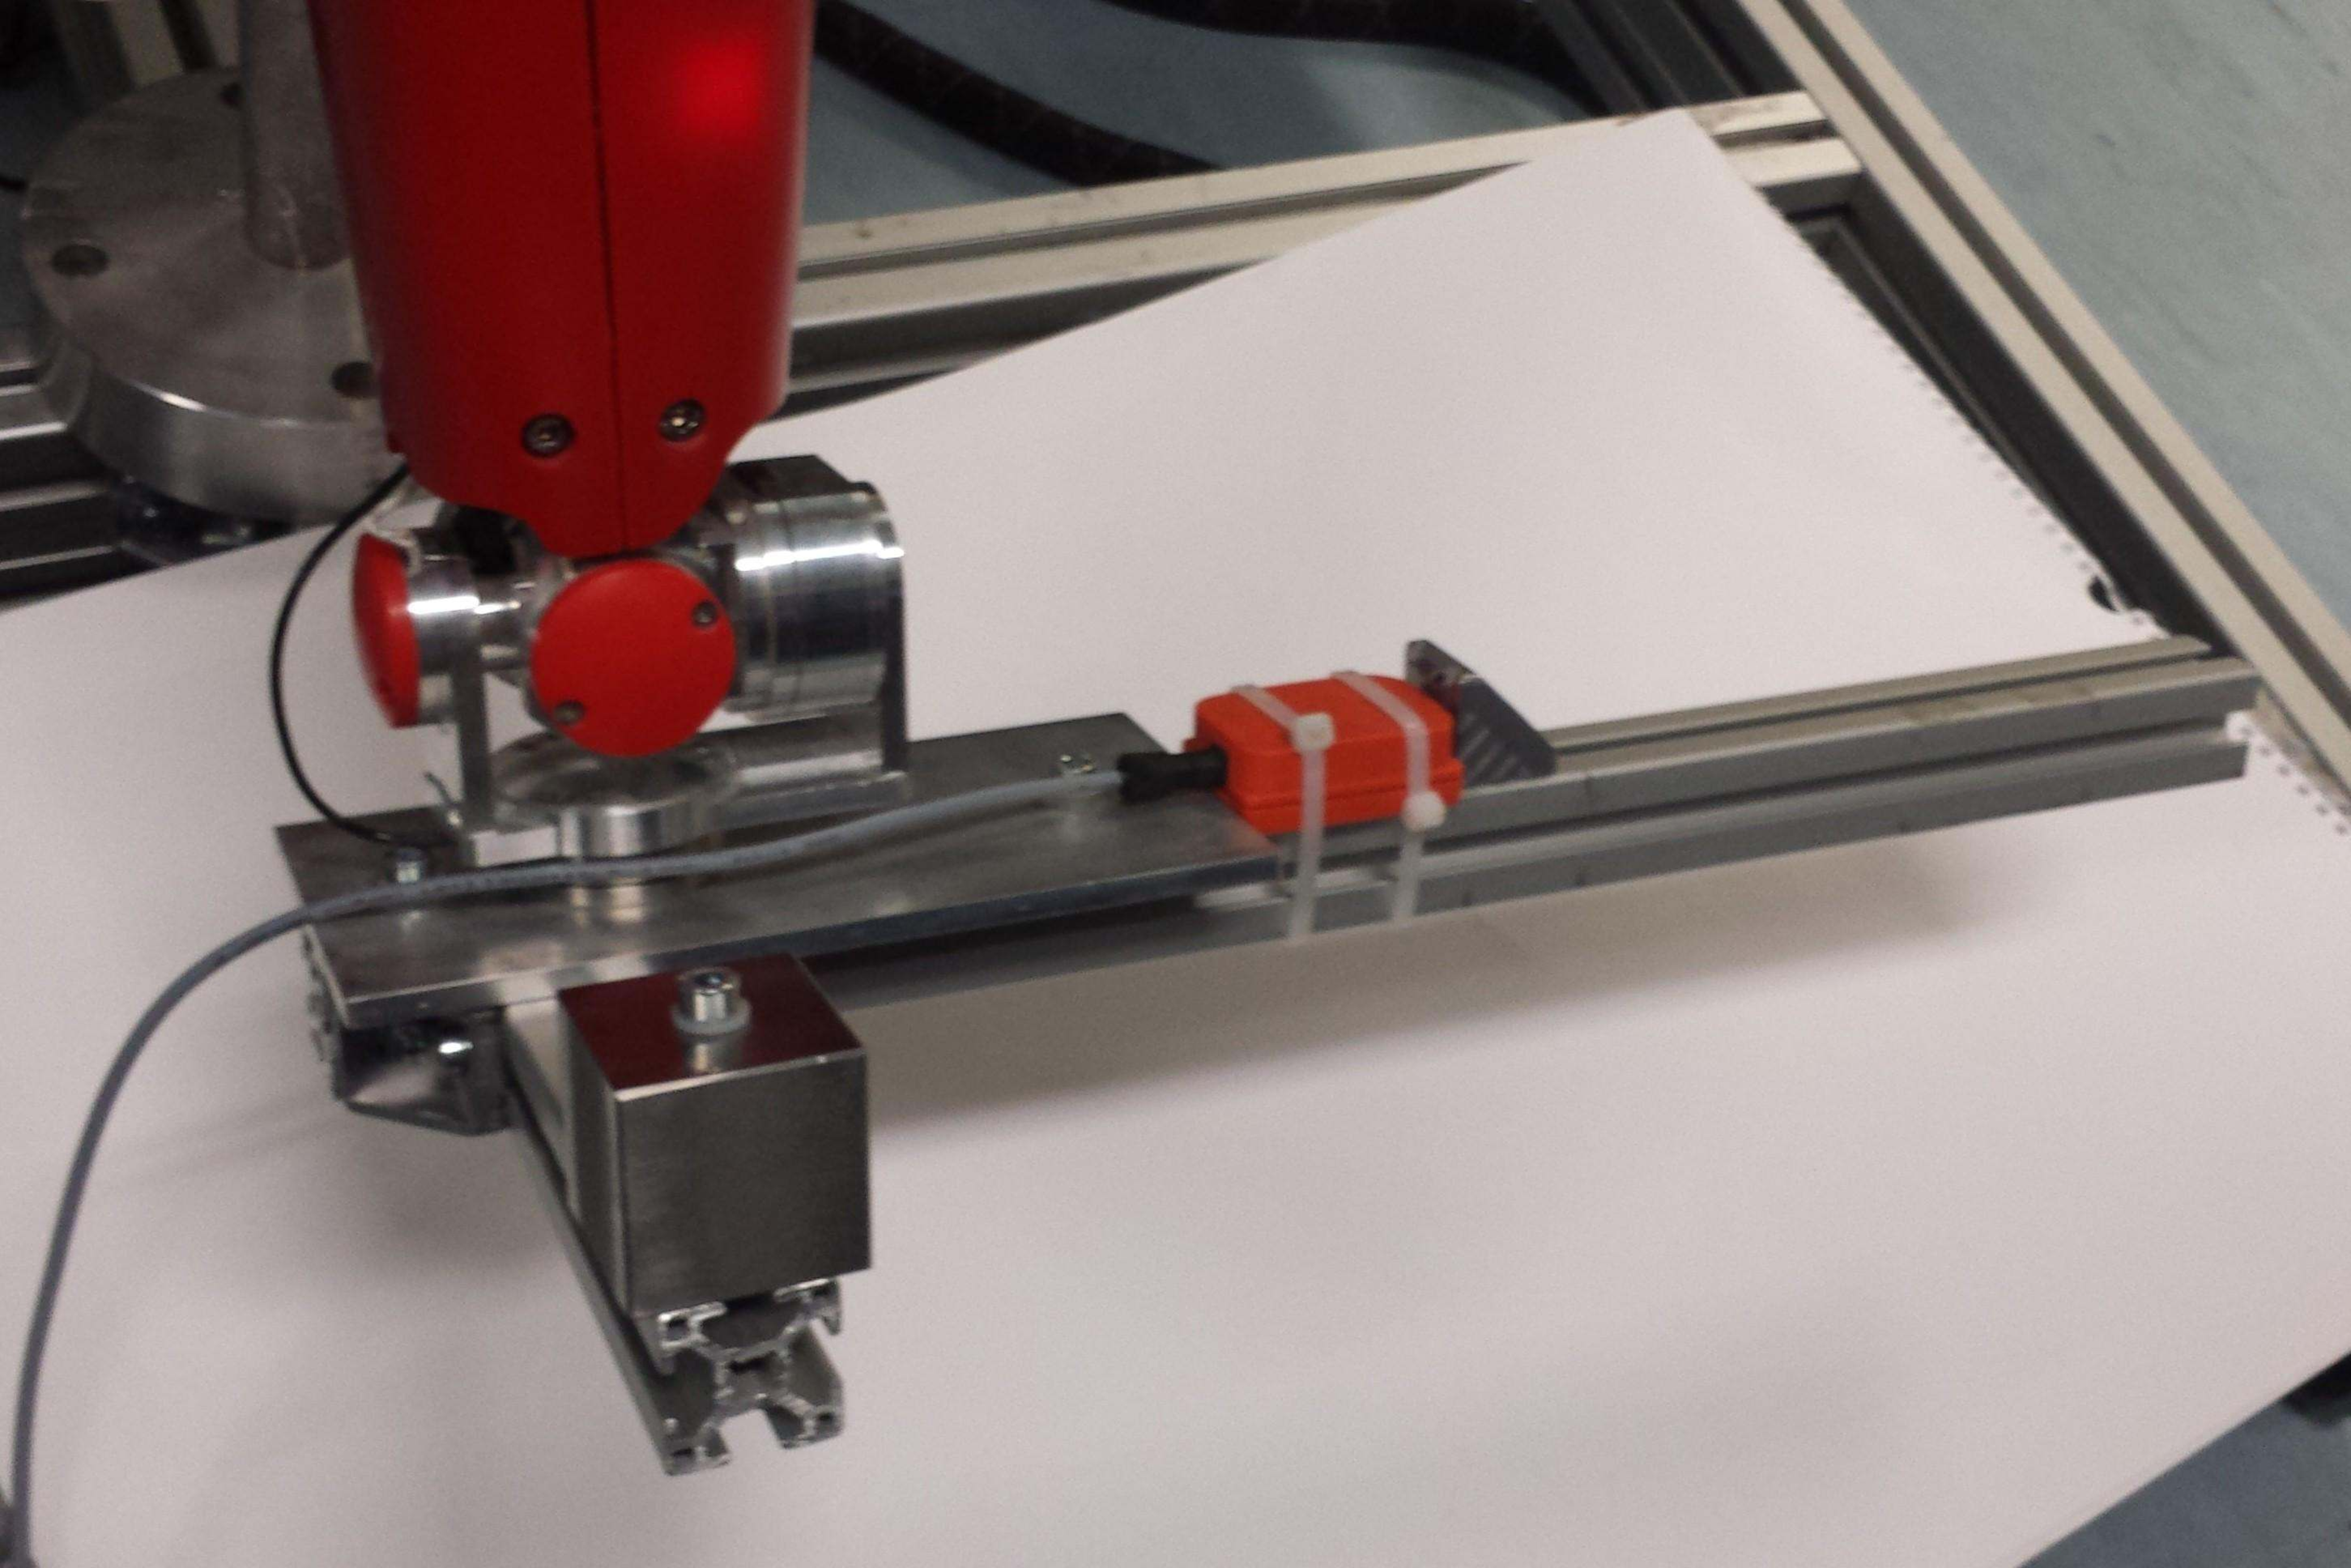
\includegraphics[width=0.22\textwidth]{images/dataset02.pdf}
\label{fig:dataset2}}
 \newline 
\subfloat[Dataset 3]{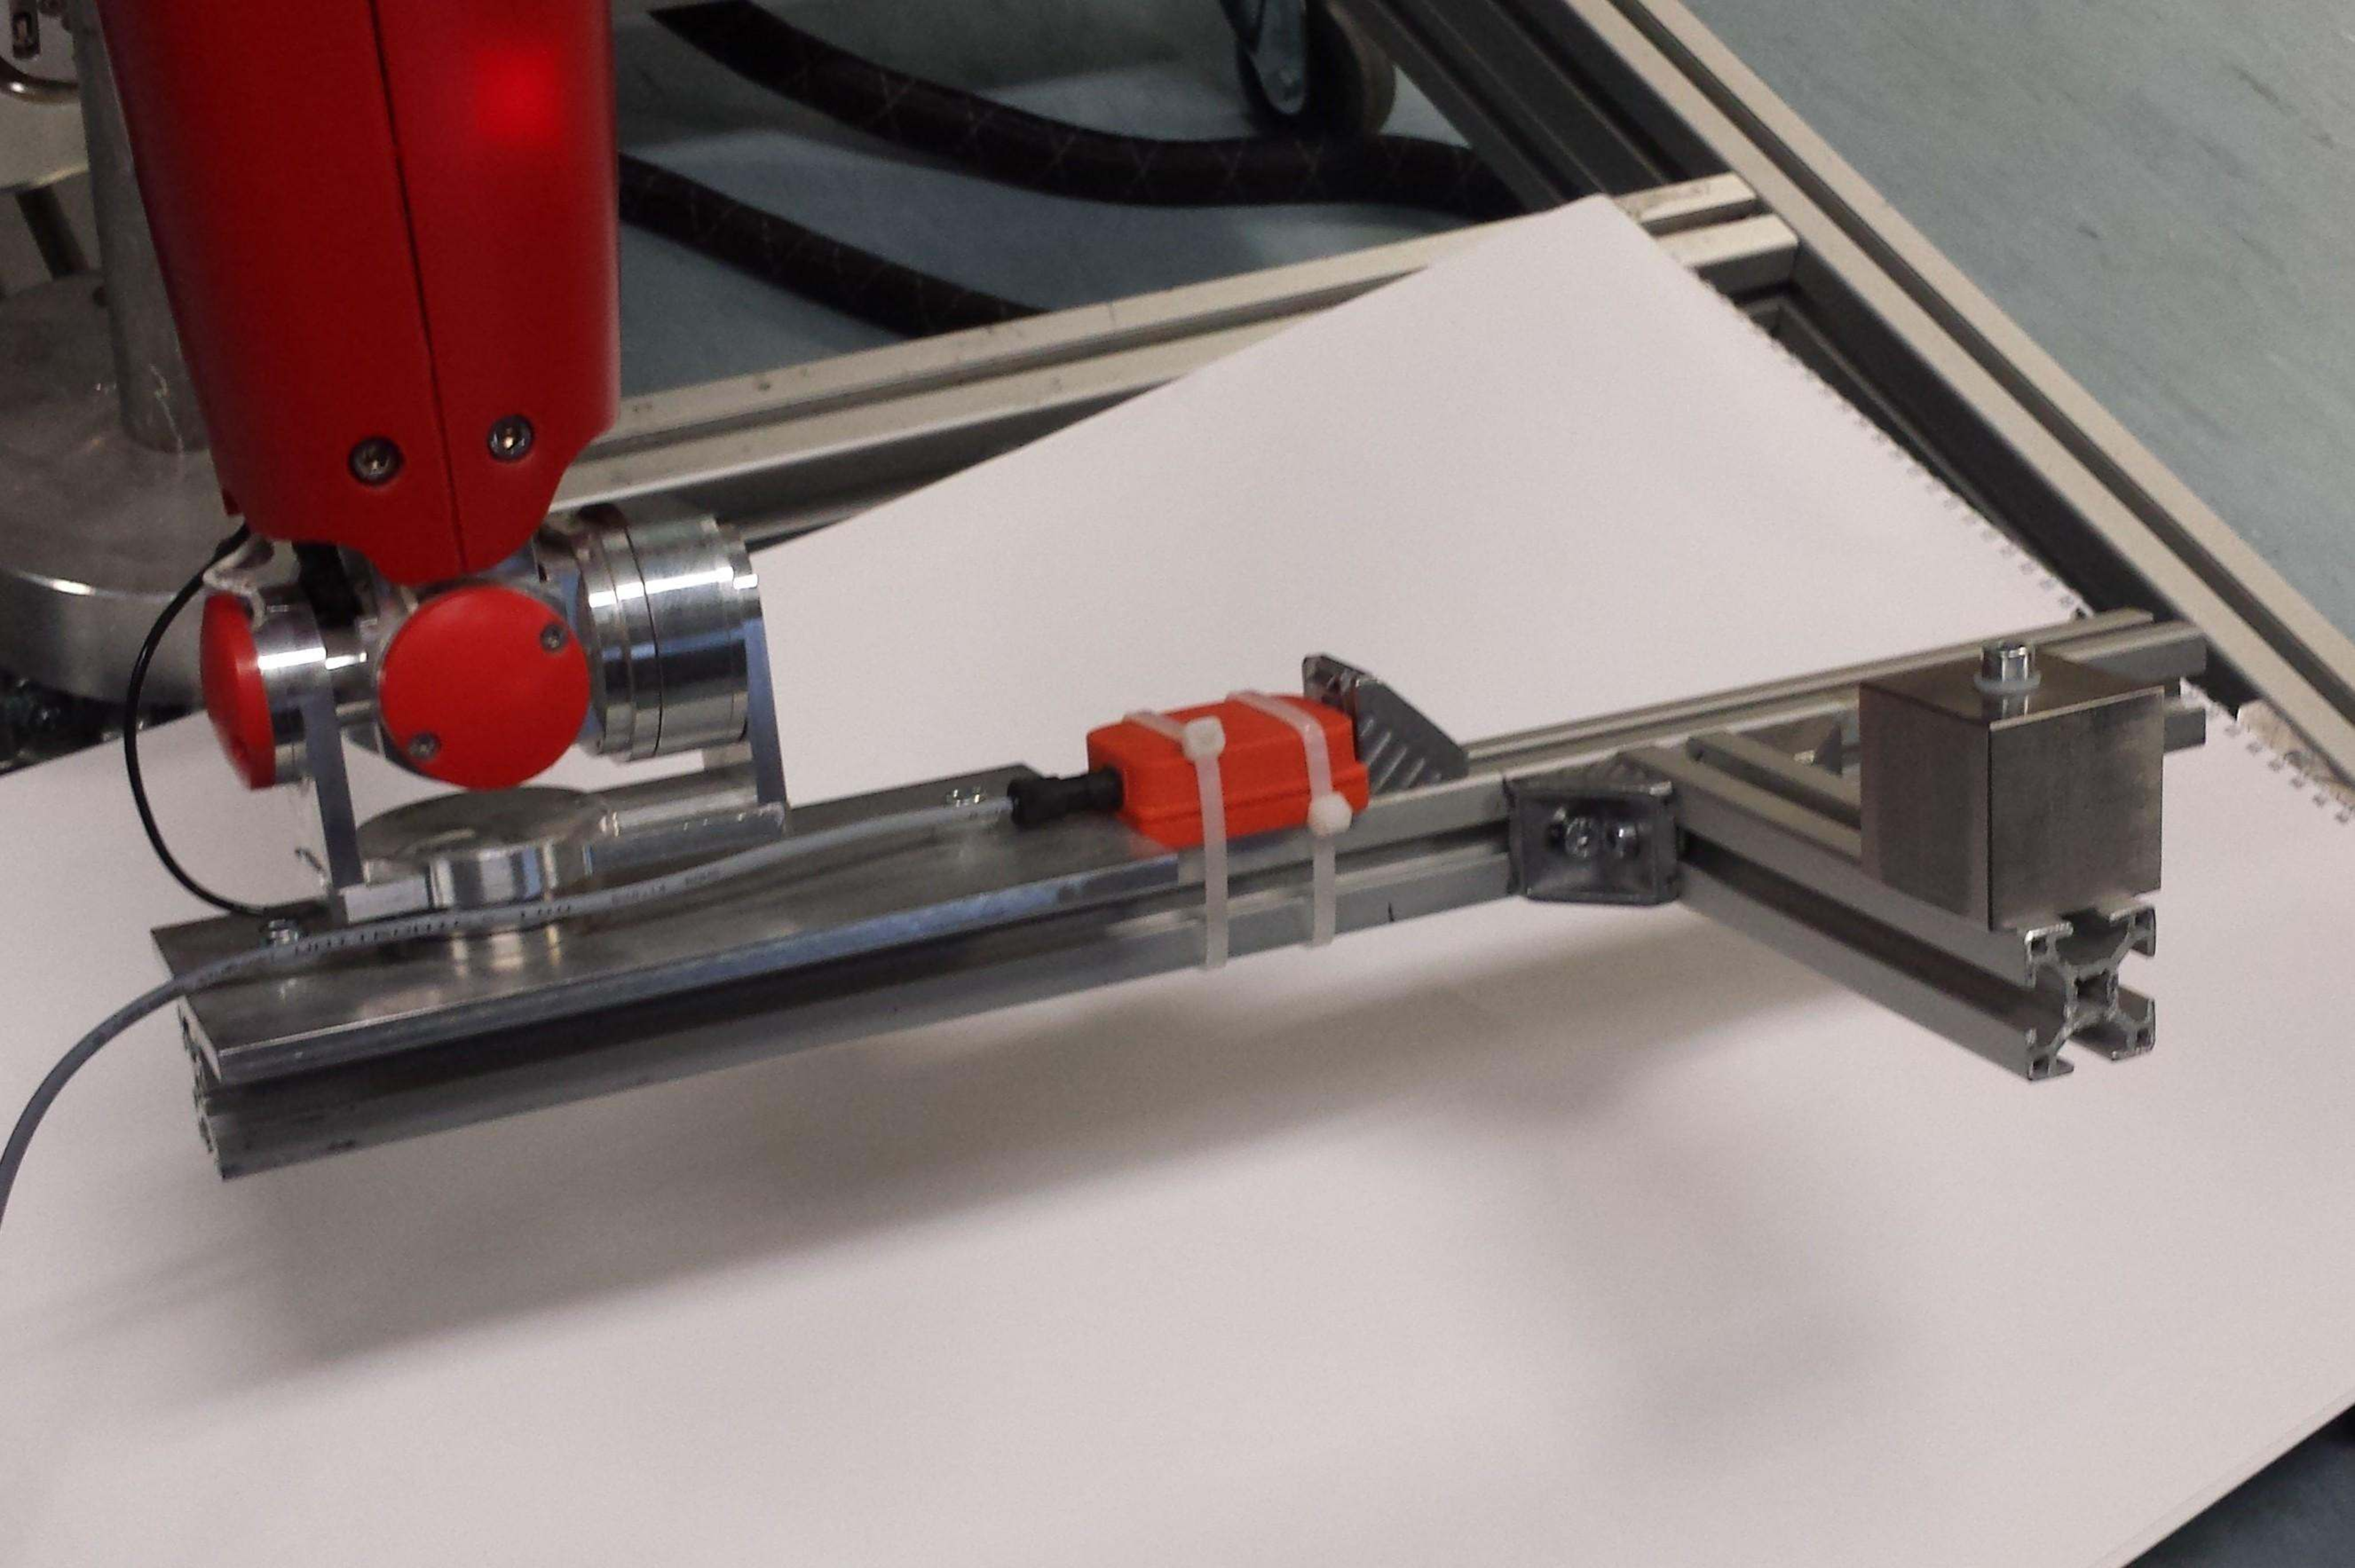
\includegraphics[width=0.22\textwidth]{images/dataset03.pdf}
\label{fig:dataset3}}
\subfloat[Dataset 4]{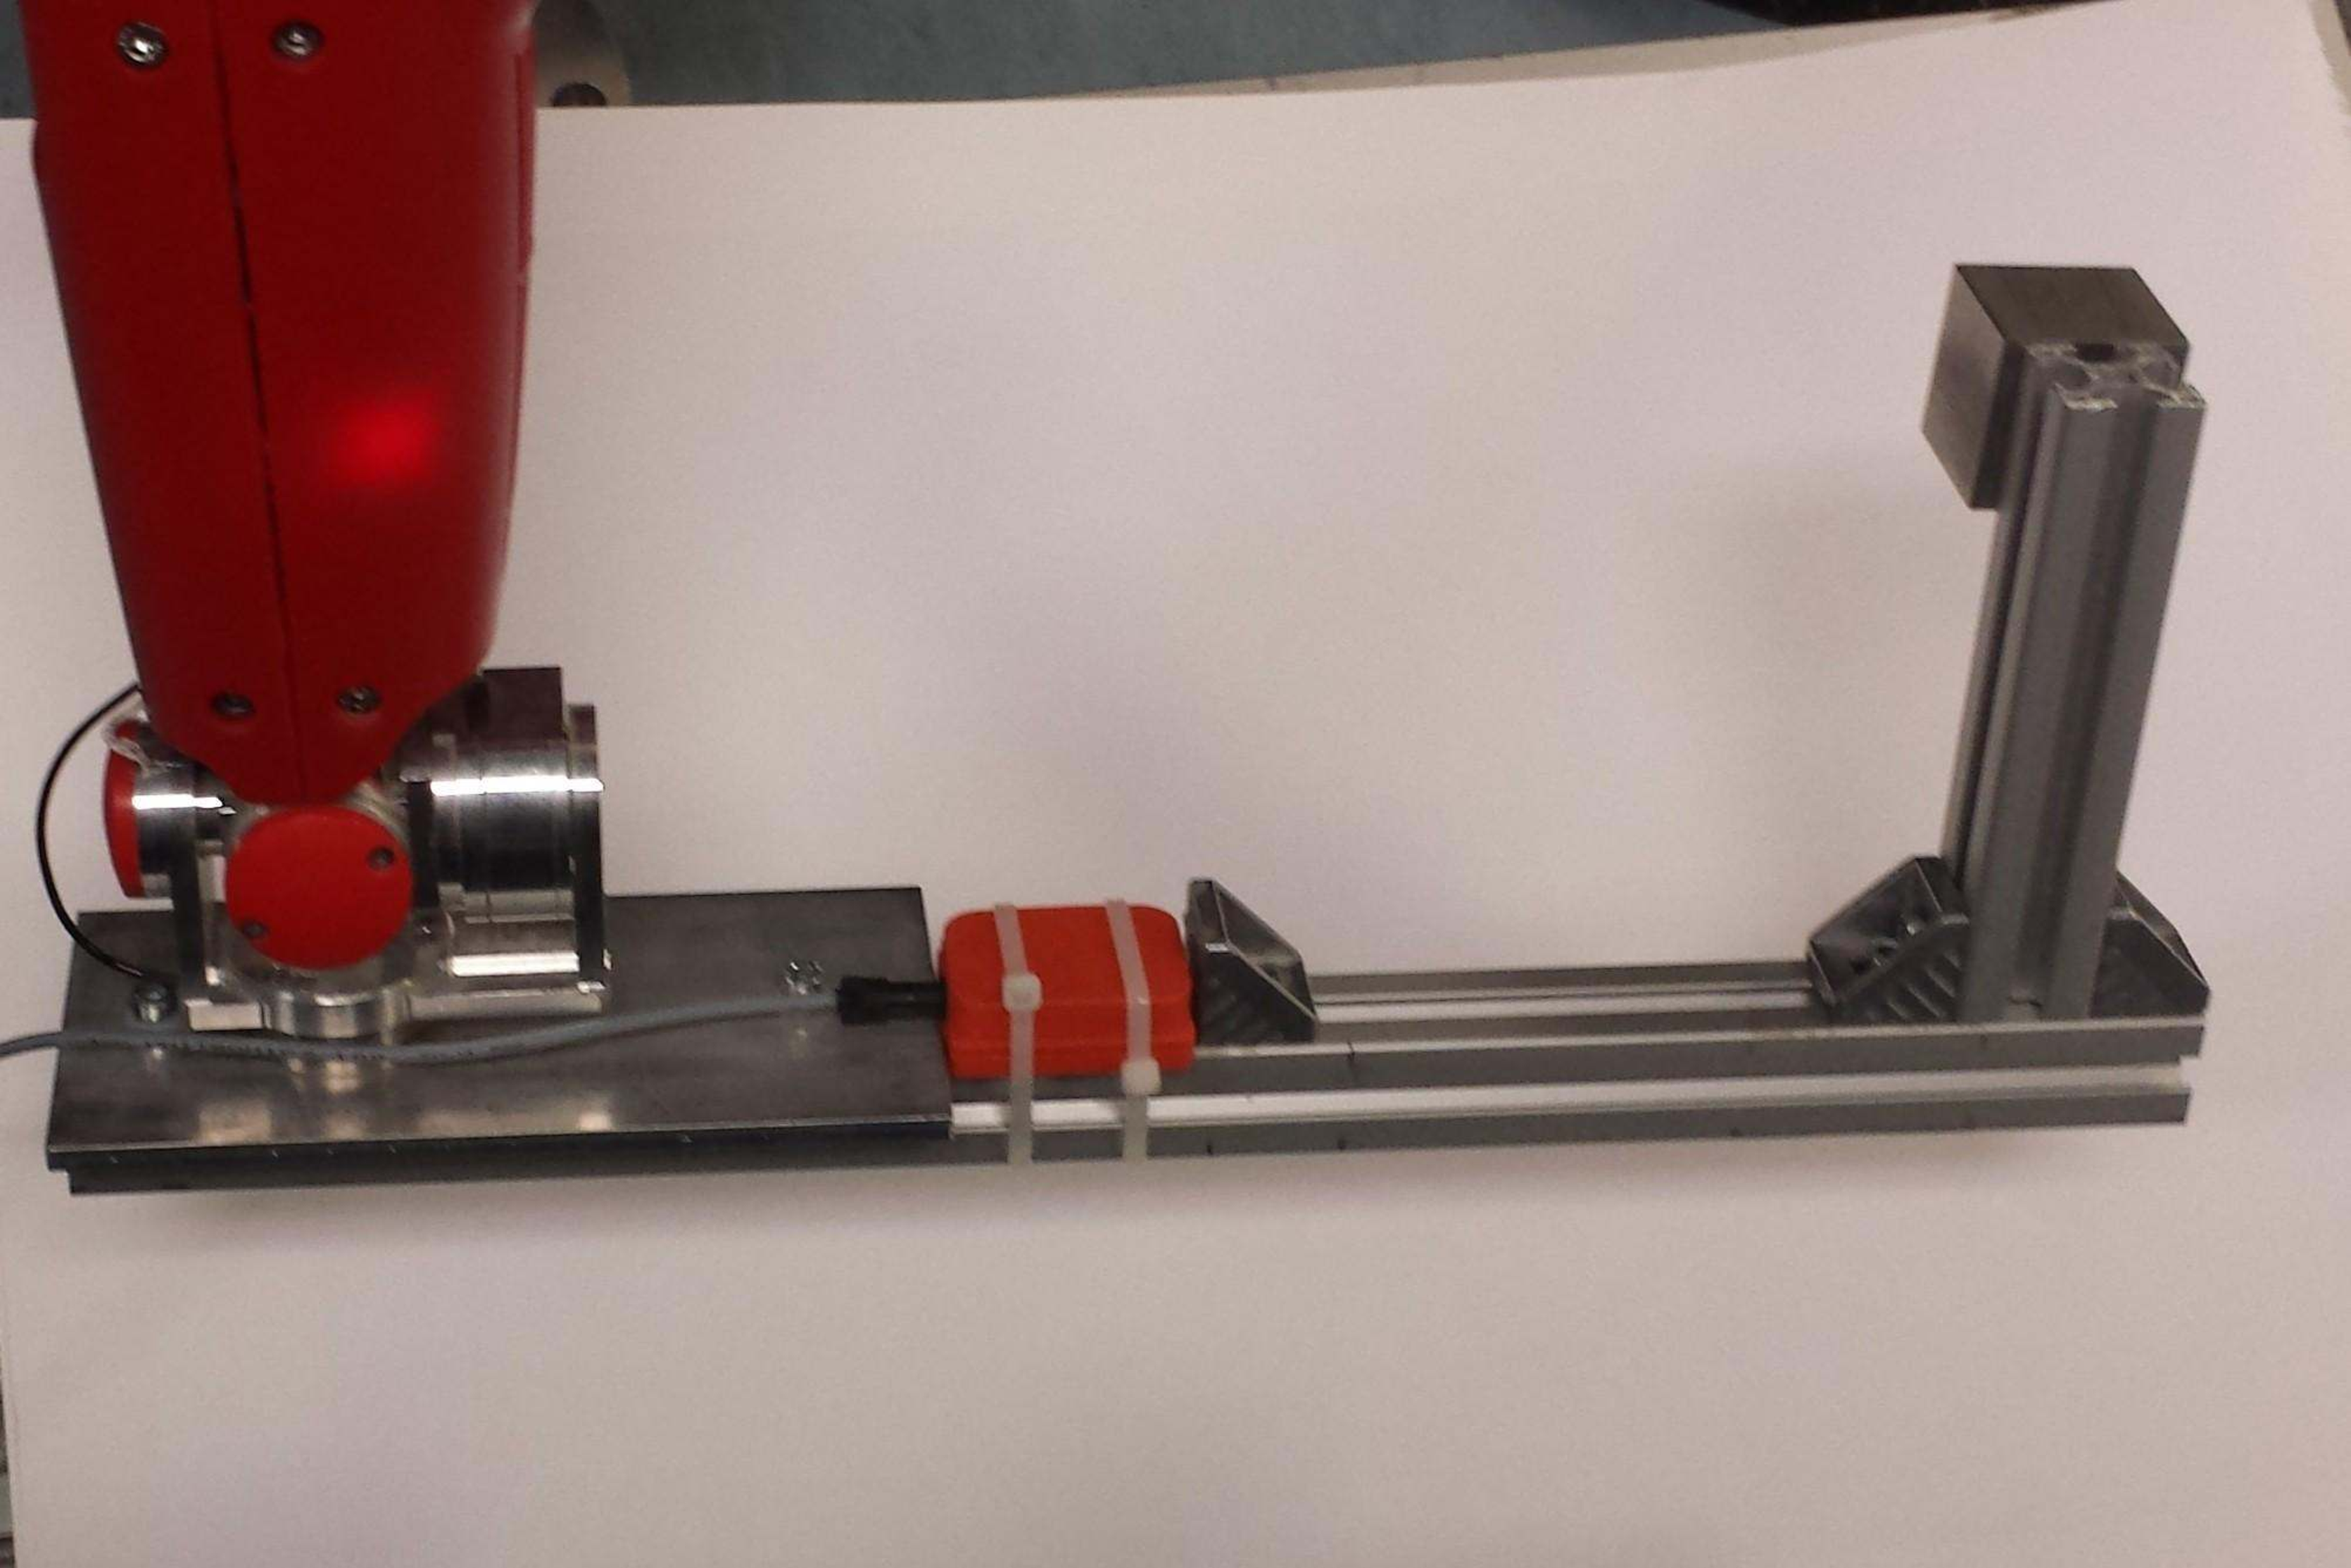
\includegraphics[width=0.22\textwidth]{images/dataset04.pdf}
\label{fig:dataset4}}
\caption{Added mass configurations for calibration datasets.}
\label{fig:calibration}
\end{figure}

\begin{proof}
This is a proof by contradiction. Assume $N_D~=~2$. In addition, assume, without loss of generality, also that the matrix $M_j$ in 
equation~\eqref{rawMeasurementsNoOffsetSeveralDataSets} 
is perfectly known (adding unknowns to the considered problem would only require a larger number of data sets). 
Then, in view of~\eqref{rawMeasurementsNoOffsetSeveralDataSets} and~\eqref{dataSets}, one has
\begin{IEEEeqnarray}{rcl}
 C(R_1,R_2) = (M_1G_1,M_2,G_2). \nonumber
\end{IEEEeqnarray}
The matrix $C$ is the unknown of the above equation. By applying \eqref{eq:kroneckerVec} one easily finds out that there exists a unique~$C$ only
if the rank of the matrix $(R_1,R_2)$ is equal to six, i.e. 
\[\text{rank}\Big( (R_1,R_2) \Big) = 6. \]
Recall that the matrix $C$ is invertible by assumption, and thus with rank equal to six. 
Consequently
\begin{IEEEeqnarray}{RCL}
 \text{rank}\Big( (R_1,R_2) \Big) &=& \text{rank}\Big( (M_1G_1,M_2,G_2)\Big) \nonumber \\
                                  &=& \text{rank}\left( (M_1,M_2)
                                  \begin{pmatrix}
                                    G_1 && 0 \\
                                    0 && G_2
                                  \end{pmatrix} \right) \nonumber \\
                                  &\leq& \min\Big(\text{rank}(M_1,M_2),6\Big).
				  \nonumber
\end{IEEEeqnarray} 
In view of~\eqref{matrixM}, one easily verifies that $\det(M_1,M_2) \equiv 0$, which implies that  \[\text{rank}\Big( (R_1,R_2) \Big) \leq 5.\] 
\end{proof}
% The proof of this lemma is straightforward and 
% % similar to the proof presented in and is 
% left to the willing reader. 

Establishing a sufficient condition for the uniqueness of the solution~$x$ to the equation~\eqref{equationForEstimatingC}
is not as straightforward as proving the above necessary condition, and is beyond the scope of the present paper. Clearly, this uniqueness is related to 
the rank of the matrix $\Theta$, and this rank condition can be verified numerically on real data.
Then, the solution~$~x$ can be found by applying least-square techniques, thus yielding estimates of the calibration matrix~$C$ and of the inertial
characteristics of the rigid body.


